\documentclass[a4paper,12pt]{article}


\usepackage{setspace}

\usepackage[T1]{fontenc} % Codificacao da fonte
\usepackage{times} % Definindo a fonte como Times New Roman

\usepackage{fancyhdr}
\pagestyle{fancy}
\lhead{Centro Universitário da FEI}

\rfoot{\thepage} %número da página
\cfoot{\textit{[ELC220] Controle Digital}}

\usepackage[left=2cm,right=2cm,top=2cm,bottom=2cm]{geometry}

\usepackage[utf8]{inputenc}


\usepackage{graphicx}
\usepackage{float}
\usepackage{amsmath}
\usepackage{gensymb}

\begin{document}
	\begin{center}
		\begin{Huge}
			Atividade Parcial
		\end{Huge}
	\end{center}

	\begin{center}
		\centering{\textbf{Gustavo Rosell Collado (11.121.526-5)}}\\
		\centering{\textbf{Massiel Blandy Ramón (11.122.397-0)}}\\
		\centering{\textbf{Thiago Travagini Moura (11.121.329-4)}}
		
		
		
	\end{center}
	
	\paragraph{}
	
	\section{Problema 1}
	Uma câmara térmica usada para testes de stress térmico em grandes equipamentos é mostrada na figura 1 com seu respectivo diagrama de blocos simplificado. Considere a unidade de tempo em minuto. A câmara é aquecida por uma linha de vapor que é controlada por uma válvula eletricamente ativa. A abertura da porta afeta a temperatura da câmara e pode ser considerada como um distúrbio. No diagrama de blocos d(t) é um distúrbio causado pela abertura da porta, e(t) é o sinal de entrada do sistema e c(t) a temperatura de saída na câmara térmica.
	

	\begin{figure}[H]
		\centering
		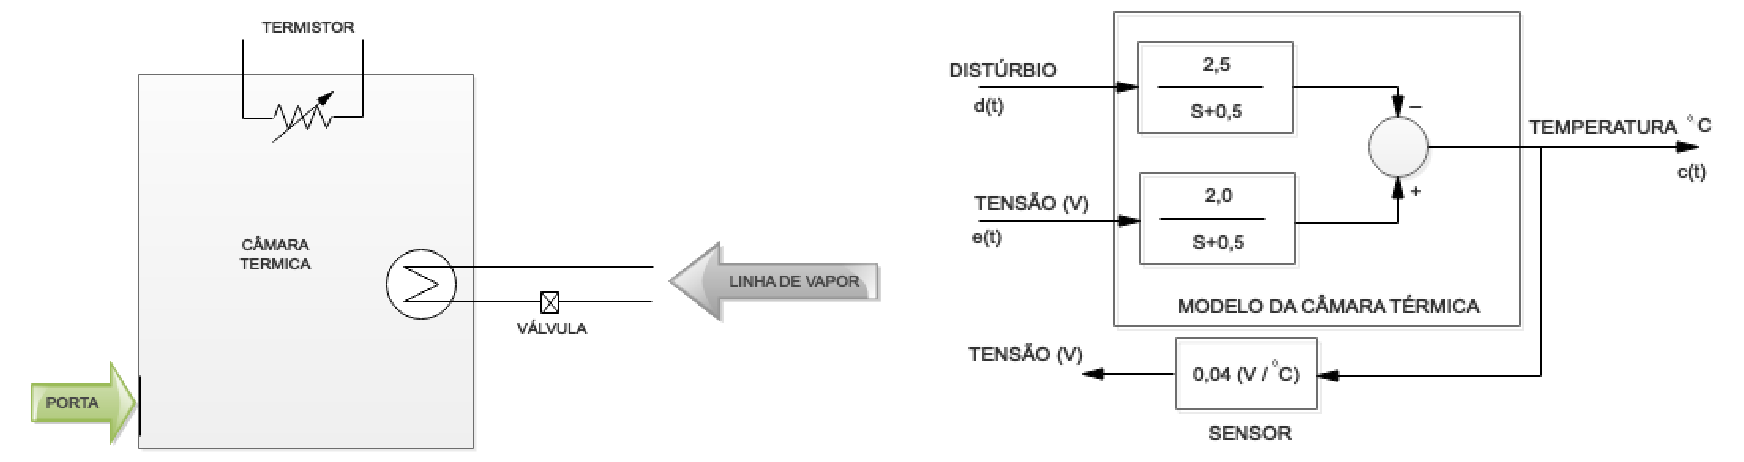
\includegraphics[width=0.9\linewidth]{images/planta_problema1}
		\label{fig:plantaproblema1}
	\end{figure}

	\subsection{Constante de tempo da câmara}
		Para analisarmos qual a constante de tempo do sistema, podemos compara-lo a forma genérica da função de sua respectiva ordem, que nesse caso é um sistema de primeira ordem. Como mostra a equação abaixo é possível obter qual a constante de tempo.
	
		\begin{equation}
			\left.
			\begin{array}{c}
				\displaystyle G(s) = \frac{K}{s+a} \\[20pt]
				\displaystyle \tau = \frac{1}{a}
			\end{array}
			\right\}
			\quad \tau = \frac{1}{0,5} = 2
		\end{equation}
	
		Portanto para a nossa câmara a constante de tempo $\tau$ é 2 minutos, portanto o tempo de subida desse ($T_s$) sistema será $4 \cdot \tau = 8$ minutos.
	
	\subsection{Resposta da câmara com condição inicial zero e sem distúrbio}
		Considerando a porta da câmara fechada (sem distúrbio) e com condição inicial 0\degree C, sendo a entrada de sinal um degrau de amplitude cinco teremos então:
		

		\begin{gather}
			C(s) = \frac{2,0}{s+0,5} \cdot \frac{5,0}{s} = \frac{10,0}{s^2 + 0,5s} = \frac{20}{s} - \frac{20}{s+0,5} \\[20pt]
			c(t) = \mathcal{L}^{-1} \{ C(s) \} = 20 + 20e^{-0,5t}
		\end{gather}
	
		Utilizando o \textit{MATLAB} foi obtido o seguinte gráfico:
		
		\begin{figure}[H]
			\centering
			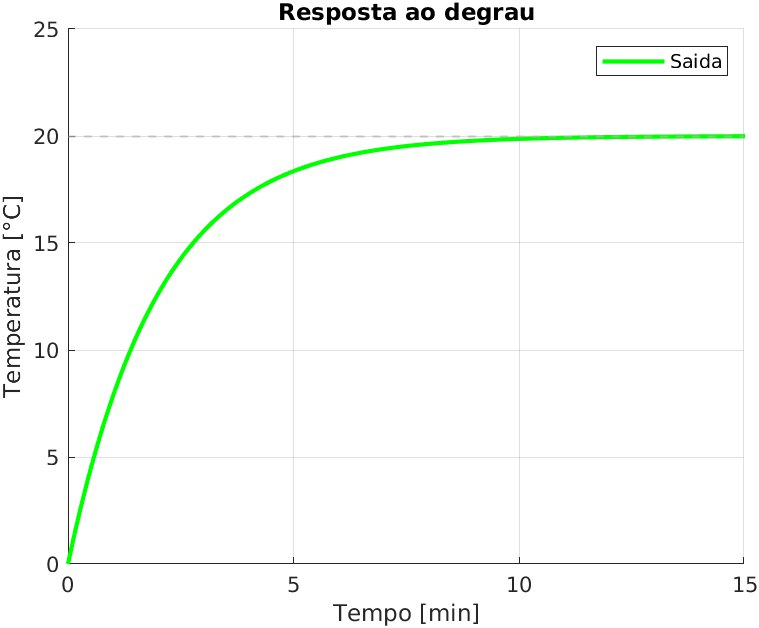
\includegraphics[width=0.5\linewidth]{images/respb.jpg}
			\label{fig:resposta_b}
		\end{figure}
	
		É possível observar que para essa entrada degrau de amplitude 5 o sistema, para $t$ tendendo ao infinito, estabilizar em 20\degree C.
		
	\subsection{Resposta da câmara com condição inicial 25\degree C e sem distúrbio}
		Sendo feita o mesmo procedimento que o item anterior, porém adicionando uma condição inicial, pode-se dizer que a única mudança será:
		
		\begin{equation}
			c(t) = c_{Anterior}(t) + x_0 \rightarrow c(t) = 45 + 20e^{-0,5t}
		\end{equation}
	
		E com essa equação temos o seguinte grafico.
		
		\begin{figure}[H]
			\centering
			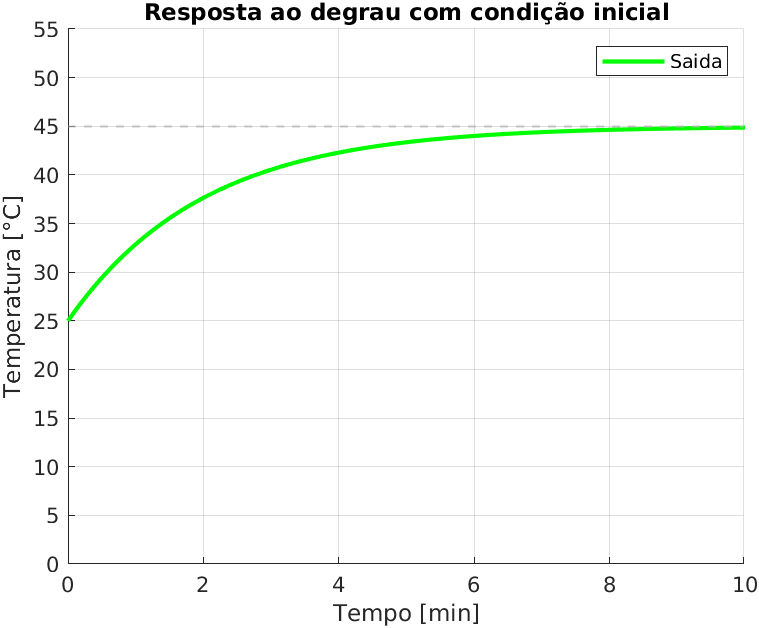
\includegraphics[width=0.5\linewidth]{images/respc.png}
			\label{fig:resposta_c}
		\end{figure}
	
	\subsection{Resposta da câmara com condição inicial 25\degree C e com distúrbio continuo}
		Nesse novo cenário é estudado como se comporta a planta para uma entrada degrau de amplitude 5, com condição inicial de 25\degree C e para um distúrbio com uma entrada de degrau unitário após 2 minutos do inicio temos que:
		
		\begin{gather}
			C(s) = G(s) \cdot E(s) - G_d(s) \cdot D(s)  + X_0(s)\\[20pt]
			C(s) = \frac{2,0}{s+0,5} \cdot \frac{5,0}{s} - \frac{2,5}{s+0,5} \cdot \frac{e^{-2s}}{s} + X_0(s) \\[20pt]
			c(t) = \mathcal{L}^{-1} \{ C(s) \} = 20 + 20e^{-0,5t} - 5e^{-0,5(t-2)}u(t-2) + 25 \\[20pt]
			c(t) = 45 + 20e^{-0,5t} - 5e^{-0,5(t-2)}u(t-2)
		\end{gather}
	
		Para essas condições a resposta do sistema foi:
		
		% TODO Ver outro nome para Planta no grafico
		\begin{figure}[H]
			\centering
			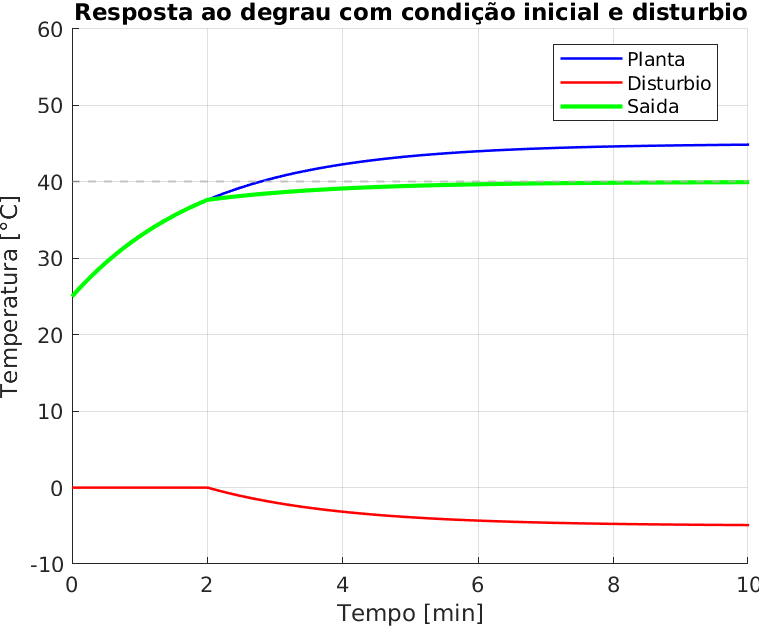
\includegraphics[width=0.5\linewidth]{images/respd.png}
			\label{fig:resposta_d}
		\end{figure}
	
		Do gráfico é possível observar o momento em que o distúrbio começa, em 2 minutos, e o valor final desse distúrbio que é de -5\degree C.
		
	% TODO: Ver outro nome para "Finito"
	\subsection{Resposta da câmara com condição inicial 25\degree C e com distúrbio}
		Nesse ultimo cenário é o mesmo utilizado acima porém com a interrupção do distúrbio apos 12 minutos do seu inicio portanto para obtermos $c(t)$ basta adicionarmos essa interrupção na resposta anterior e a função sera:
		
		\begin{equation}
			c(t) = 45 + 20e^{-0,5t} - 5e^{-0,5(t-2)}u(t-2) + 5e^{-0,5(t-14)}u(t-14)
		\end{equation}
	
		E sua resposta foi:
		
		% TODO Ver outro nome para Planta no grafico
		% TODO Arrumar acentos
		\begin{figure}[H]
			\centering
			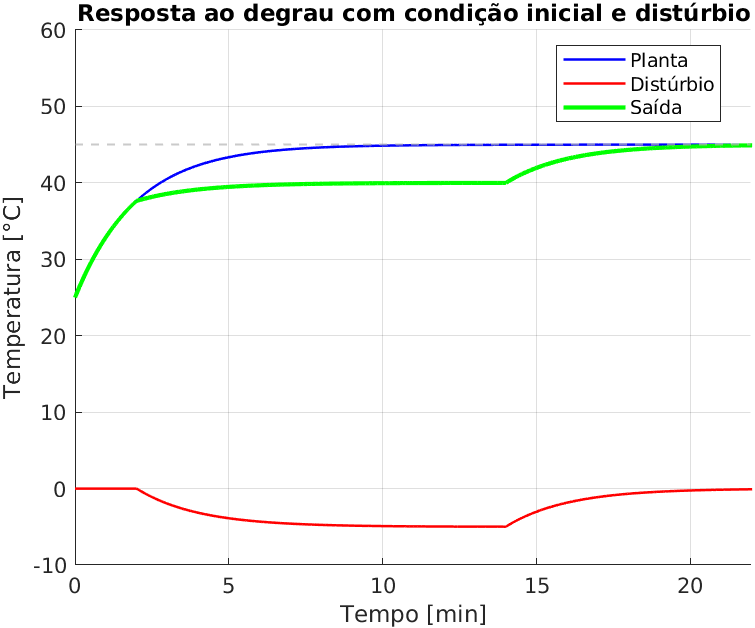
\includegraphics[width=0.5\linewidth]{images/respe.png}
			\label{fig:resposta_e}
		\end{figure}
		
		
		
		
		
		
		
		
	
	
\end{document}